

% \begin{filecontents*}{main_NAT_experiments.csv}
% Window Size,"1,1","2,2","4,4","8,8","0,1","0,2","0,4","0,8"
% distilled data from scratch,27.04,25.48,22.52,18.13,26.94,25.76,23.55,19.63
% distilled data from pretrained,27.44,25.75,22.72,16.7,26.37,26.45,23.87,19.5
% original data from scratch,26.14,22.58,16.92,7.18,26.12,23.26,18.72,9.45
% original data from pretrained,26.27,23.1,17.15,6.85,23.57,23.41,18.18,9.45
% \end{filecontents*}


Inspired by the abovementioned in Section \ref{subsec:transfer_learning}, we present our suggested approach and model architecture. 


\section{Past and Future N-gram Language Modeling Task} \label{sec:past_future_n-gram_lm}

\begin{figure}[hpbt!]

    \centering
    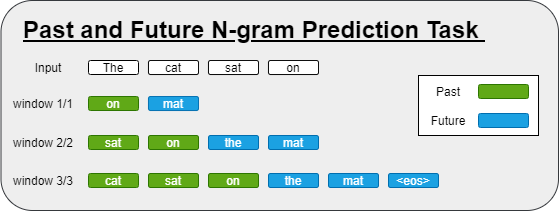
\includegraphics[width=\textwidth]{images/chap04_images/ngram language modeling.png}
    \caption{An example of the Past and Future N-gram Language modeling task. The model predicts a past window and a future window given the input.}
    \label{fig:n-gram_lm}
\end{figure}

We introduce a variant of the N-gram prediction task \cite{qi_prophetnet_2020}. In the Past and Future Language Modeling task, the model is trained to predicted a window size of tokens. An example is shown in \ref{fig:n-gram_lm}. The configuration of the window is specified by the user. For simplicity, we set the window sizes to be powers of 2. Half of the window is used to predict past tokens, and the other half is used to predict the future tokens. 

There are several reasons behind this design. Firstly, predicting past tokens allows us to do sequence refinement (as mentioned in Section \ref{subsec:sol5_post_editing}), while speeding up generation. A window size of 1/1 (Future window of 1 and back window of 1) defaults to autoregressive generation while allowing the capability for post editing. A window size of 4/4 (Future window of 4 and back window of 4) speeds up generation by 4x relative to autoregressive generation. We also experiment with non-uniform window sizes; such as 4/2 (future window size of 2 and past window size of 4). Secondly, this enable us to utilize the autoregressive decoding framework without having to reinvent the wheel and significantly introduce changes in the model. Decoding of a sequence can halt when there is an end of sequence token generated in the future window. Lastly, this objective is straightforward, and allows for transfer learning from autoregressive models.

\section{Model Architecture}\label{sec:architecture}

\begin{figure}[hpbt!]

    \centering
    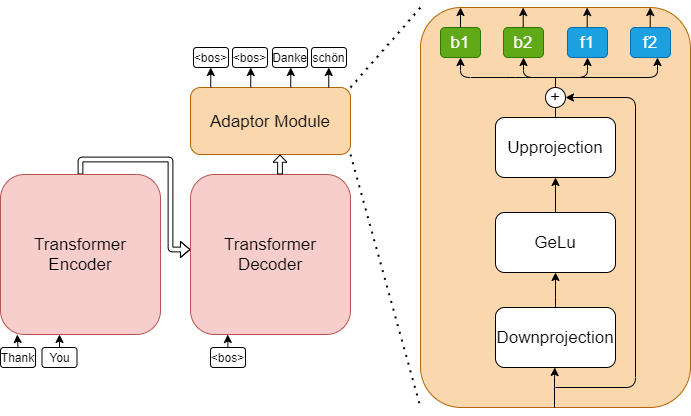
\includegraphics[width=\textwidth]{images/chap04_images/adaptor_module.png}
    \caption{Model Architecture. The transformer encoder and decoder is kept the same. We append the adaptor module to the output of the transformer decoder. In this example, the window size of model is 2/2 (past window of 2 and future window of 2).}
    \label{fig:AT_vs_NAT}
\end{figure}

We keep the transformer architecture the same. However, instead of applying a softmax over the last hidden state in the decoder, we pass all hidden states to the adaptor module. The adaptor module is adapted from \textcite{houlsby_parameter-efficient_2019_adaptor2}. The hidden states are down-projected to a hidden size of a specified hyperparameter, passed through the non-linearity GeLu, and then up-projected back to the original hidden size. A residual connection is used to add the original hidden states to the up-projection. This architecture is simple and allows for transfer learning to be done using publicly available models.

\section{Decoding Methods} \label{sec:decoding_methods}
Typically, beam search is used for decoding in autoregressive models. Other non-autoregressive methods like the Levenshtein Transformer \cite{gu_levenshtein_2019} are unable to use beam search as beam search requires a contiguous beam of tokens to be scored at each decoding step. Therefore, most non-autoregressive models rely on Noisy Parallel Decoding \cite{gu_non-autoregressive_2018}, which uses an autoregressive model to score each translation. However, this is somewhat inefficient for practical reasons as the whole idea of non-autoregressive research is to streamline decoding without having to rely on autoregressive methods. 

\begin{figure}[hpbt!]

    \centering
    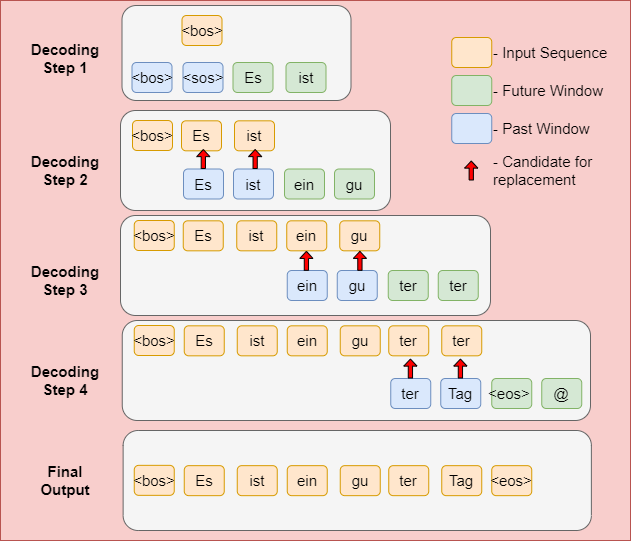
\includegraphics[width=\textwidth]{images/chap04_images/decoding.png}
    \caption{An example of decoding for a window size of 2/2 (2 future and 2 past). At each decoding step, two future tokens from the future window size of 2 are added to the sequence. The two tokens from the past prediction window are candidates for sequence refinement. In this example at decoding step 4, 'Tag' from the past window replacement replaces the duplicate 'ter' in the already generated sequence.The generation halts when there is an end of sequence token, and all tokens after the end of sequence token are ignored.}
    \label{fig:decoding_example}
\end{figure}

Our architecture does allows us to reuse the methods of autoregressive decoding. This can be done in several ways. The first way is by predicting the future window, similar to that in autoregressive decoding. Every step, the next window of tokens will be predicted, and added to the output. There are two terminating conditions for the sequence generation. The first terminating condition is when any of the tokens in the future output prediction window is the end of sequence token. The second terminating condition is the when there has been too many decoding iterations. In reality, the second terminating condition almost never triggers due to the speed of decoding.

In each decoding method, we will first explain the process of decoding for the future prediction window, followed by how it is applied using the past prediction window to sequence refinement. The general decoding process is illustrated in Figure \ref{fig:decoding_example}.

\subsection{Argmax Decoding} \label{subsec:argmax_decoding}
Argmax Decoding a greedy decoding method which is straightforward and easy to to apply. For the future window prediction, the most probable token in the output distribution for each window slot is taken as the generated sequence. For the future window prediction, the probable token is taken as the candidate token.

For sequence refinement, argmax decoding also chooses the most probable token in each window slot in the past prediction window as the candidate tokens. However, the already generated sequence is only replaced by its overlapping window slot if the probability of the candidate token is higher than the probability of the incumbent token. This requires us to keep a history of probabilities for each token, which is non-trivial to implement practically.

\subsection{Hysteresis Decoding} \label{subsec:hysteresis_decoding}
We present a new decoding method called Hysteresis Decoding. Hysteresis Decoding is inspired by hysteresis edge tracking from the field of computer vision.

\begin{figure}[hpbt!]
    \centering
    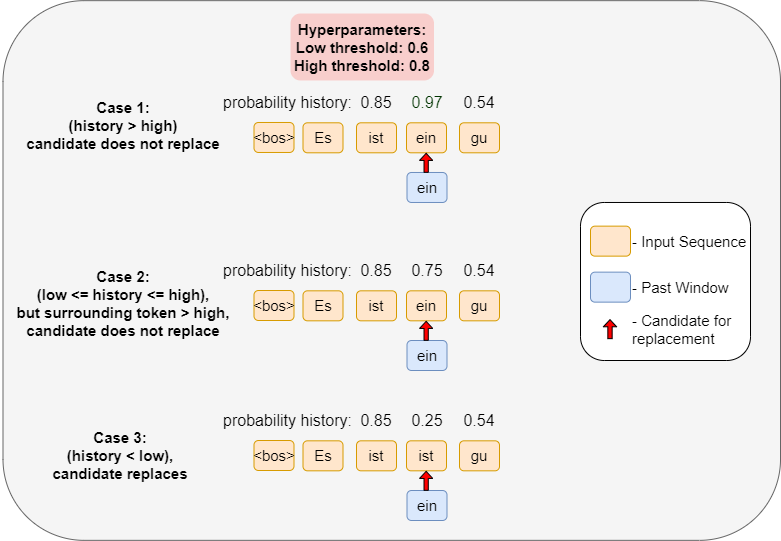
\includegraphics[width=\textwidth]{images/chap04_images/hysteresis_decoding.png}
    \caption{An example of how hysteresis decoding works. Low and high probability thresholds are 0.6 and 0.8. Each token in the previously generated sequence will be strong, weak, or low, depending on its probability history. If the probability is greater than the high threshold, it is a strong token. If the probability is between the high and low thresholds, it is a weak token. If the probability is less than the low threshold, it is a low token. \textbf{Case 1:} Previously generated token has a probability history of 0.97. Since the probability of the previously generated token is higher than the high probability threshold, it is assigned as a strong token and the the candidate token will not replace it. \textbf{Case 2:} Previously generated token has a probability history of 0.75. It is greater than the low threshold but lower than the high threshold. Therefore, the previously generated token is a weak token. However, there is a surrounding token on the left which is a strong token because it has a probability threshold of 0.85. Therefore, the candidate token will not replace it. \textbf{Case 3:} The previously generated token has a probability of 0.25. It is less than the low threshold, therefore it is a low token and the candidate token will replace it.}
    \label{fig:hysteresis_decoding_ex}
\end{figure}

In our experiments, hysteresis decoding is only applied to sequence refinement for the past prediction window. Theoretically, it can also be used for the future window prediction, but argmax decoding works well for the future window prediction without the need for hysteresis decoding. Hysteresis decoding refers to the suppression of the candidate token if the probability of the surrounding tokens (ie. the tokens on the left and right tokens) are low. Conversely, if the probability of a surrounding token is higher than the high threshold, the candidate token will be accepted and replace. This process is depicted in Figure \ref{fig:hysteresis_decoding_ex}, along with an example. Currently, there are two ways to determine the low and high threshold. The first way is via a prespecified probability range based on the probability of the candidate token. The second way is via a prespecified low and high probability threshold, both of which are hyperparameters. 

\subsection{Beam Search}


Beam search is a popular decoding method and often works in complement with other greedy decoding methods. Beam search works by expanding the search space of the decoding process in exchange for increased computational and memory requirements.  Beam search is often used together with argmax decoding.


\section{Implementation Details} \label{sec:implementation_details}
% Always use vectorized graphics. Black and white plots with different markerstyles \textgreater multicolor plots 
We use the fairseq library\footnote{https://github.com/pytorch/fairseq} for implementation. The dataset used is the WMT14 En-De dataset, which has been helpfully preprocessed and provided by fairseq\footnote{https://github.com/pytorch/fairseq/tree/master/examples/nonautoregressive\_translation} as well. Both the original and distilled datasets are used in our experiments.

First, we train an original transformer using the specified steps for 300k iterations using the original WMT14 En-De dataset. We try to keep the number of words per batch to around 25000, but practically, the number of words per batch range between 23000 and 27000 depending on the amount of GPU memory available. After training the original transformer, we average the last 10 trained checkpoints, and then use the averaged checkpoint as the pretrained model for transfer learning in training non-autoregressive models. We use the same dictionary to process both distilled and original data.

For other hyperparameters, we set learning rate to 0.0005 using the adam optimizer with a inverse square root learning rate schedule along with a 10000 warmup update. The lowest learning rate that can be set by the optimizer is $1e^{-09}$. We use label smoothed cross entropy and share all embeddings.

We reuse the same hyperparameters for our experiments when training the non-autoregressive models. The hidden layer size for our adaptor module is 64. We train our models in several settings to compare the effects. First, to compare the effect of transfer learning for non-autoregressive sequence generation, we train models both from scratch and from the pretrained model. Secondly, to compare the effect of the past and future n-gram prediction task, we train models with the past and future n-gram prediction task, and models with only the future n-gram prediction task. We also examine the effect of the past and future n-gram prediction task by turning off the past window during decoding. Last, we freeze layers by turning off backpropagation to those layers in the transformer during transfer learning to see how it impacts the training.

When evaluating and performing inference with our models, we use a variety of decoding methods. Unless stated, the default decoding method is argmax decoding. Other decoding methods used includes beam search and hysteresis decoding. As per the standard in non-autoregressive machine translation, we use the BLEU4 score as the evaluation metric.


\section{N-gram Prediction Experiments} \label{sec:n-gram_experiments}
As mentioned in Section \ref{sec:ngram_lm}, we use the N-gram prediction task for n-gram prediction. The size of the future prediction window affects how fast the decoding proceeds. For example, a future prediction window of 1 defaults to autoregressive decoding, while a future prediction window of 8 allows us to generate 8 tokens in a forward pass, therefore resulting in a speed up of 8. On the other hand, a past prediction window allows us to perform iterative refinement. A past window size of 1 allows us to refine the last token in the already generated sequence, while a past window size of 8 allows us to refine the past 8 tokens in already generated sequence. We first compare the effect of only predicting the future n-grams, and the effect of predicting both past and future n-gram. 

We experiment with varying window sizes for n-gram prediction. These window sizes go from 1 to 8, in intervals of power of 2. While there is propensity for using unequal future and past window sizes, for instance future window size of 8 and past window size of 4, we show results with only equal window sizes for now.

\section{Comparing the effect of the past-future n-gram prediction task and the future n-gram prediction}

We trained models of varying window sizes with the past-future n-gram prediction task, along with its counterpart model without any past prediction window. This is to compare the effectiveness of the prediction task in training the models. Our results are shown in Table \ref{tab:4.4_past_future_vs_future}.

\begin{table}[]
\begin{tabular}{cc|c|c|c|c|c|c|c|c|}
\cline{3-10}
\multicolumn{1}{l}{}                                                          & \multicolumn{1}{l|}{}                                         & \multicolumn{8}{c|}{past or future window size}                     \\ \cline{3-10} 
\multicolumn{1}{l}{}                                                          & \multicolumn{1}{l|}{\textbf{}}                                & \multicolumn{4}{c|}{from scratch} & \multicolumn{4}{c|}{pretrained} \\ \hline
\multicolumn{1}{|c|}{\begin{tabular}[c]{@{}c@{}}training\\ task\end{tabular}} & \begin{tabular}[c]{@{}c@{}}sequence\\ refinement\end{tabular} & 1      & 2      & 4      & 8      & 1      & 2      & 4     & 8     \\ \hline
\multicolumn{1}{|c|}{past-future}                                             & yes                                                           & 27.04  & 25.48  & 22.52  & 18.13  & 27.44  & 25.75  & 22.72 & 16.7  \\ \hline
\multicolumn{1}{|c|}{past-future}                                             & no                                                            & 26.94  & 25.5   & 22.65  & 18.89  & 27.44  & 25.78  & 22.88 & 17.66 \\ \hline
\multicolumn{1}{|c|}{future-only}                                             & no                                                            & 26.94  & 25.76  & 23.55  & 19.63  & 26.37  & 26.45  & 23.87 & 19.5  \\ \hline
\end{tabular}
\caption{Each row compares the BLEU4 score of models trained on the past-future n-gram prediction task. The first row and second row uses the same model for decoding, the difference being sequence refinement is not used when decoding in the second row. The last row refers to the model being trained on future n-gram prediction only. The window sizes refer to the past or future window size. For example, window size of 4 for past-future n-gram prediction means that past window size is 4, and future window size is 4. On the other hand, window size of 4 for future only n-gram prediction task means that the future window size is 4, while the past window size is 0.}
\label{tab:4.4_past_future_vs_future}
\end{table}


\subsection{Effectiveness of argmax sequence refinement} \label{subsec:effective_argmax}
We compare the effectiveness of argmax sequence refinement on models trained with the past-future n-gram prediction task, with models trained on the future-only n-gram prediction task. As explained in Section \ref{sec:past_future_n-gram_lm}, the past window provides the opportunity for sequence refinement. However, the trade off is that there is added difficulty for the model as the model has to learn to predict both past and future tokens. From our experiments, models decoded with argmax sequence refinement (1st row of Table \ref{tab:4.4_past_future_vs_future}) do not perform better the models without sequence refinement (2nd and 3rd row of Table \ref{tab:4.4_past_future_vs_future}). We hypothesize that the argmax decoding is insufficient and too naive for sequence refinement. Therefore we introduced hysteresis decoding, as mentioned in Section \ref{fig:hysteresis_decoding_ex}.


\subsection{Effectiveness of the past-future n-gram prediction task}
In this section, we compare the effectiveness of the past-future n-gram prediction without sequence refinement to the future-only n-gram prediction task (2nd and 3rd row of Table \ref{tab:4.4_past_future_vs_future}). This is done by ignoring the past prediction window during decoding of the model. From our experiments, the inclusion of the past window for prediction during training did not seem to benefit the performance of the model. While the difference in BLEU score were insignificant for lower windows sizes 1 and 2, the disparity in the BLEU score grew as the window sizes increased.




\section{Influence of transfer learning on different types of data}
\textcite{gu_non-autoregressive_2018} asserted that the use of distilled data was instrumental in helping non-autoregressive models learn better. Hence we also perform a suite of experiments on both distilled and original data. As mentioned earlier in Section \ref{sec:implementation_details}, both distilled and original data were provided by fairseq. We perform all experiments on both distilled and original data. Our results are shown at Table \ref{tab:4.5_distill_vs_original_results}.


\begin{table}[]
\begin{tabular}{cc|cccc|cccc|}
\cline{3-10}
\multicolumn{1}{l}{}                                & \multicolumn{1}{l|}{} & \multicolumn{8}{c|}{Past/Future window size}                  \\ \cline{3-10} 
                                                    &                       & 1/1   & 2/2   & 4/4   & 8/8   & 0/1   & 0/2   & 0/4   & 0/8   \\ \hline
\multicolumn{1}{|c|}{\multirow{2}{*}{from scratch}} & distill               & 27.04 & 25.48 & 22.52 & 18.13 & 26.94 & 25.76 & 23.55 & 19.63 \\
\multicolumn{1}{|c|}{}                              & original              & 26.14 & 22.58 & 16.92 & 7.18  & 26.12 & 23.26 & 18.72 & 9.45  \\ \hline
\multicolumn{1}{|c|}{\multirow{2}{*}{pretrained}}   & distill               & 27.44 & 25.75 & 22.72 & 16.7  & 26.37 & 26.45 & 23.87 & 19.5  \\
\multicolumn{1}{|c|}{}                              & original              & 26.27 & 23.1  & 17.15 & 6.85  & 23.57 & 23.41 & 18.18 & 9.45  \\ \hline
\end{tabular}
\caption{Each row shoes the BLEU4 score of each model. Models of the same model configurations but trained on different data are grouped together. Each column corresponds to the past-future n-gram prediction window size of the model. For example, 2/2 means the past and future n-gram prediction window size are both 2, which 0/2 means there is no past n-gram prediction window, and only a future n-gram prediction window of 2.}
\label{tab:4.5_distill_vs_original_results}
\end{table}


\subsection{Effectiveness of transfer learning}
In our experiments, using pretrained models for transfer learning yield slightly better BLEU4 scores at smaller windows sizes 1, 2 and 4, but the benefits diminishes with increased window size 8. The improvement from using a pretrained model over training from scratch is shown in Figure \ref{fig:difference_bleu_pretrained_from_scratch}.

%plot difference in bleu4 score for transfer learning
\begin{figure}
\centering
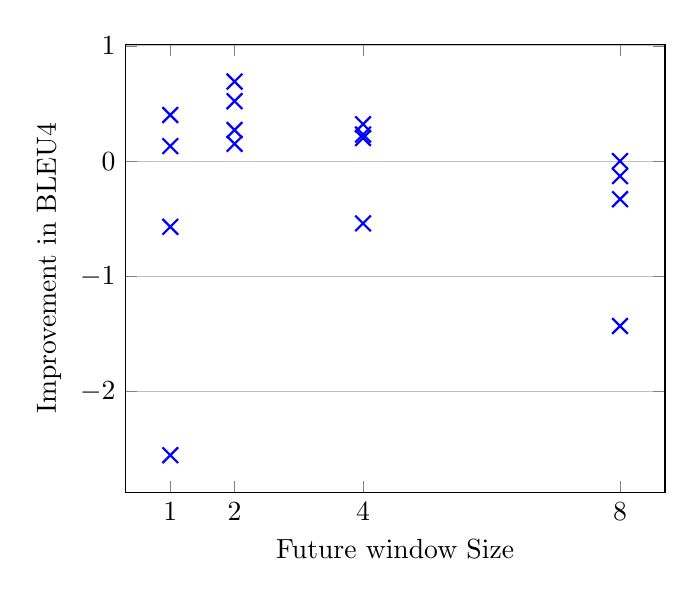
\begin{tikzpicture}
\begin{axis}[
    xlabel={Future window Size},
    ylabel={Improvement in BLEU4},
    xtick={0,1,2,4,8},
    ymajorgrids=true,
    % grid style=dashed,
]

\addplot[
    color=blue,
    mark=x,
    only marks,
    thick,
    mark size=4pt
    ]
    coordinates {
    (1, 0.4)(1, 0.13)(1,-0.57)(1,-2.55)(2,0.27)(2,0.52)(2,0.15)(2,0.69)(4,0.2)(4,0.23)(4,0.32)(4,-0.54)(8,0)(8,-0.13)(8,-1.43)(8,-0.33)
    };
    
\end{axis}
\end{tikzpicture}
\caption{Magnitude of improvement in BLEU4 scores between models trained from a pretrained model over training from scratch. We group models based on their future n-gram prediction window sizes. For example, for a model trained on past-future n-gram prediction of window size 2 for both past and future, the model trained from a pretrained model had an improvement of 0.52 over the model trained from scratch}
\label{fig:difference_bleu_pretrained_from_scratch}
\end{figure}

\subsection{Effectiveness of using sequence level knowledge distillation}
As collaborated in many other work in non-autoregressive literature \cite{ren_study_2020_comma, gu_non-autoregressive_2018, gu_levenshtein_2019, guo_non-autoregressive_2020_image_captioning, bao_non-autoregressive_2019_position_learning, wang_semi-autoregressive_2018,saharia_non-autoregressive_2020_latent_alignment, chan_kermit_2019, chan_multilingual_kermit, ghazvininejad_mask-predict_2019,stern_insertion_2019, zhou_improving_2020_with_monolingual_data, ran_guiding_2020_reordering, ma_flowseq_2019, qian_glancing_2020, guo_fine-tuning_2019_curriculum, ding_context-aware_2020}, models trained on distilled data for non-autoregressive machine translation performed significantly better than original data. From our experiments, the difference in BLEU4 score between the model trained on distilled data and its model counterpart trained on original data assumes an almost linear relationship. This relationship is shown in Figure \ref{fig:difference_bleu_distill_original}. 

%plot difference in bleu4 score
\begin{figure}
\centering
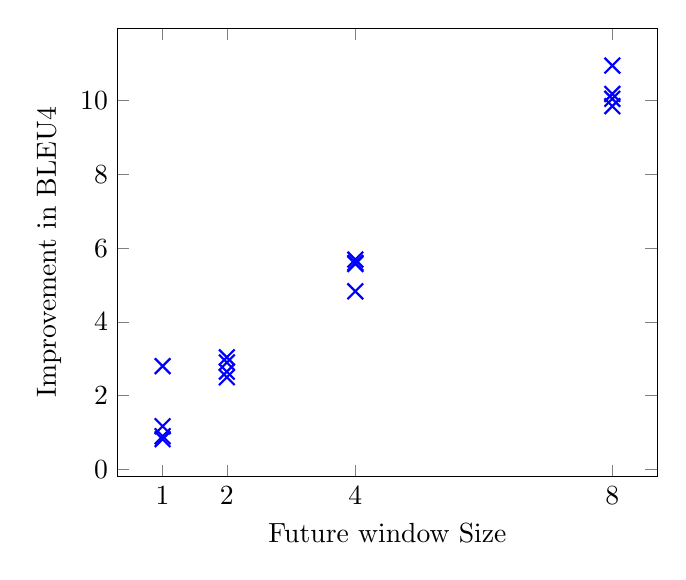
\begin{tikzpicture}
\begin{axis}[
    xlabel={Future window Size},
    ylabel={Improvement in BLEU4},
    xtick={0,1,2,4,8},
    % ymajorgrids=true,
    % grid style=dashed,
]

\addplot[
    color=blue,
    mark=x,
    only marks,
    thick,
    mark size=4pt
    ]
    coordinates {
    (1, 0.9)(1,1.17)(1,0.82)(1,2.8)(2,2.9)(2,2.65)(2,2.5)(2,3.04)(4,5.6)(4,5.57)(4,4.83)(4,5.69)(8,10.95)(8,9.85)(8,10.18)(8,10.05)
    };
    
\end{axis}
\end{tikzpicture}
\caption{Magnitude of improvement in BLEU4 scores between models trained on distilled over original data. We group models based on their future n-gram prediction window sizes. For example, for a model trained on past-future n-gram prediction of window size 4 for both past and future, the model trained on distilled data achieved an improvement of 5.6 in BLEU score.}
\label{fig:difference_bleu_distill_original}
\end{figure}



\section{Effect of Decoding Methods} 
As noted in Section \ref{sec:decoding_methods}, we use several methods for decoding during inference. These methods include argmax decoding, beam search of beam length 1 to 4, and hysteresis decoding.

\subsection{Argmax Decoding}
Argmax Decoding is the most straightforward decoding method. In our experiments, unless stated, argmax decoding is the default method. At each decoding step, the most probable token(s) is chosen as the generated token. Our results using argmax decoding are shown in Table \ref{tab:4.5_distill_vs_original_results}. Argmax decoding works well for the prediction of the future window. However, as noted in Section \ref{subsec:effective_argmax}, argmax decoding is too naive for sequence refinement. Therefore, we introduce hysteresis decoding for sequence refinement.

\subsection{Beam Search}
Beam search also consistently improves the BLEU score across all settings. Beam search can also be used in complement with both argmax decoding and hysteresis decoding. Take note that beam size of 1 is equivalent to simple argmax decoding. We show the results for models trained on distilled data, without any sequence refinement, at Table \ref{tab:beam_search_results_npe}. 

\begin{table}[]
\centering
\begin{tabular}{|c|c|c|cccc|}
\hline
\begin{tabular}[c]{@{}c@{}}Future \\ Window Size\end{tabular} & setting      & training task & beam1 & beam2 & beam3 & beam4  \\ \hline
8                                                             & from scratch & past-future   & 18.89 & 19.03 & 19.09 & 19.09  \\ \cline{3-7} 
8                                                             & from scratch & future-only   & 19.63 & 19.73 & 19.77 & 19.78  \\ \cline{2-7} 
8                                                             & pretrained   & past-future   & 17.66 & 18.08 & 18.17 & 18.19  \\ \cline{3-7} 
8                                                             & pretrained   & future-only   & 19.50  & 19.67 & 19.72 & 19.73  \\ \hline
4                                                             & from scratch & past-future   & 22.65 & 23.05 & 23.12 & 23.19  \\ \cline{3-7} 
4                                                             & from scratch & future-only   & 23.55 & 23.73 & 23.79 & 23.82  \\ \cline{2-7} 
4                                                             & pretrained   & past-future   & 22.88 & 23.18 & 23.28 & 23.3   \\ \cline{3-7} 
4                                                             & pretrained   & future-only   & 23.87 & 23.82 & 23.87 & 23.9   \\ \hline
2                                                             & from scratch & past-future   & 25.50  & 25.73 & 25.84 & 25.84  \\ \cline{3-7} 
2                                                             & from scratch & future-only   & 25.76 & 25.8  & 25.85 & 25.883 \\ \cline{2-7} 
2                                                             & pretrained   & past-future   & 25.78 & 26.01 & 26.11 & 26.13  \\ \cline{3-7} 
2                                                             & pretrained   & future-only   & 26.45 & 26.57 & 26.6  & 26.59  \\ \hline
1                                                             & from scratch & past-future   & 27.01 & 27.11 & 27.27 & 27.35  \\ \cline{3-7} 
1                                                             & from scratch & future-only   & 26.94 & 27.29 & 27.41 & 27.37  \\ \cline{2-7} 
1                                                             & pretrained   & past-future   & 27.44 & 27.61 & 27.6  & 27.54  \\ \cline{3-7} 
1                                                             & pretrained   & future-only   & 26.37 & 26.47 & 26.49 & 26.49  \\ \hline
\end{tabular}
\caption{BLEU4 scores of models decoded using argmax decoding and beam search of size 1, 2, 3 and 4, and without doing sequence refinement. Future window size refers to the window size of the future n-gram prediction. Setting refers to the model being trained from scratch, or from a pretrained model using transfer learning. Training task refers to the task the model is trained on, which is either the past-future n-gram prediction task, or the future-only n-gram prediction task.}
\label{tab:beam_search_results_npe}
\end{table}

\begin{figure}[hpbt!]
    \centering
    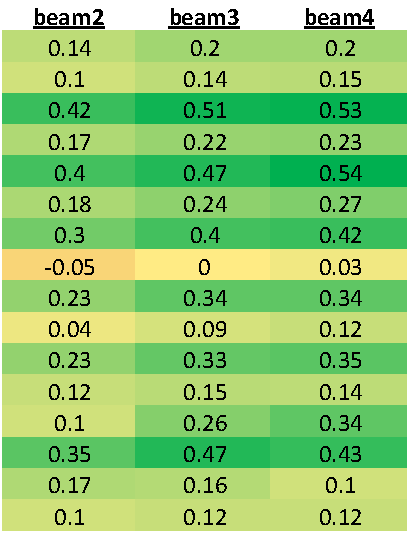
\includegraphics{images/chap04_images/beam_search_improvements.pdf}
    \caption{Improvement of BLEU4 score over beam size 1 when using a higher beam length 2, 3, 4. The darker the shade of green, the higher the improvement. For example, the model in the first row has an improvement of 0.14 in BLEU4 when decoding with beam search 2.}
    \label{fig:beam_search_improvement}
\end{figure}

From our experiments, beam search of increasing beam sizes performs consistently better than when using beam size of 1. These improvements in performance is depicted using color coding in Figure \ref{fig:beam_search_improvement}.

\subsection{Hysteresis Decoding} 
As previously introduced in Section \ref{subsec:hysteresis_decoding}, Hysteresis decoding is a decoding method aimed to improve sequence refinement using the past prediction window of the n-gram prediction task. There are two settings for which we can perform hysteresis decoding, by using a range, or by tweaking the low and high thresholds of the hysteresis decoding.


\subsubsection{Range Hysteresis Decoding} \label{subsubsec:range_hdec}

\begin{figure}[hpbt!]
    \centering
    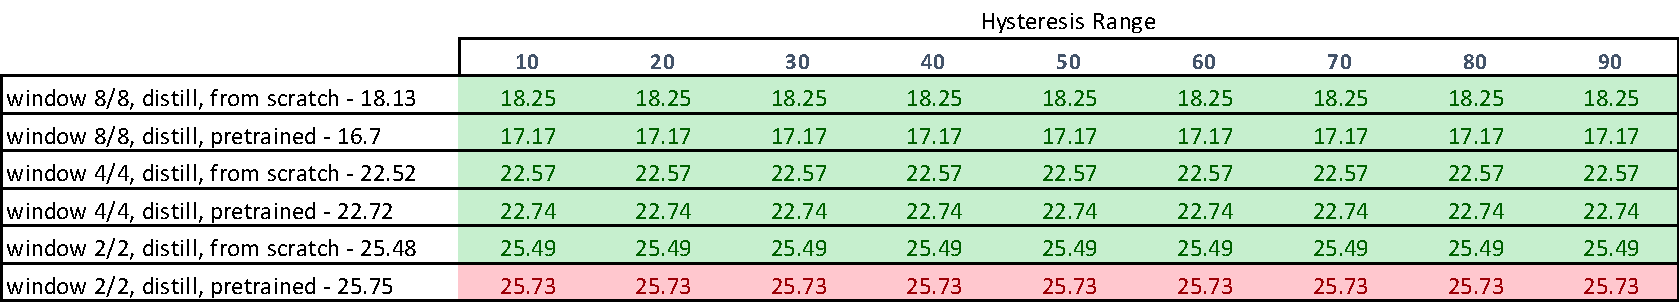
\includegraphics[width=\textwidth]{images/chap04_images/hysteresis_decoding_range.pdf}
    \caption{BLEU4 score of models decoded using the range setting. For example, a model trained from scratch on 8/8 past and future n-gram prediction task on distilled data scored a BLEU4 score of 18.25, an improvement over its argmax decoding BLEU4 score of 18.13.}
    \label{fig:hysteresis_decoding_range}
\end{figure}

We use a range from 0.1 to 0.9 in intervals of 0.1. For example, if the hysteresis range is 0.2, and the probability of the candidate token is 0.50, the low and high threshold will be 0.30 and 0.70 respectively. We cap the highest and lowest probabilities to be compared against the candidate probability to be 0.95 and 0.05 respectively. This is to prevent the probabilities from going over 1.00 or under 0.


Our results are shown in Figure \ref{fig:hysteresis_decoding_range}. There is a clear benefit of BLEU score when using hysteresis decoding for large window sizes of 16. However, benefit seems to be reduced for smaller window sizes. Furthermore, the performance of the hysteresis decoding method seems to be independent from how wide the probability range is. Aside from a model trained on small window sizes (2/2), all models in our experiments yielded positive improvements when using range hysteresis decoding for sequence refinement.

\subsubsection{Manually setting high-low thresholds for Hysteresis Decoding} \label{subsubsec:manual_hdec}

\begin{figure}[hpbt!]

    \centering
    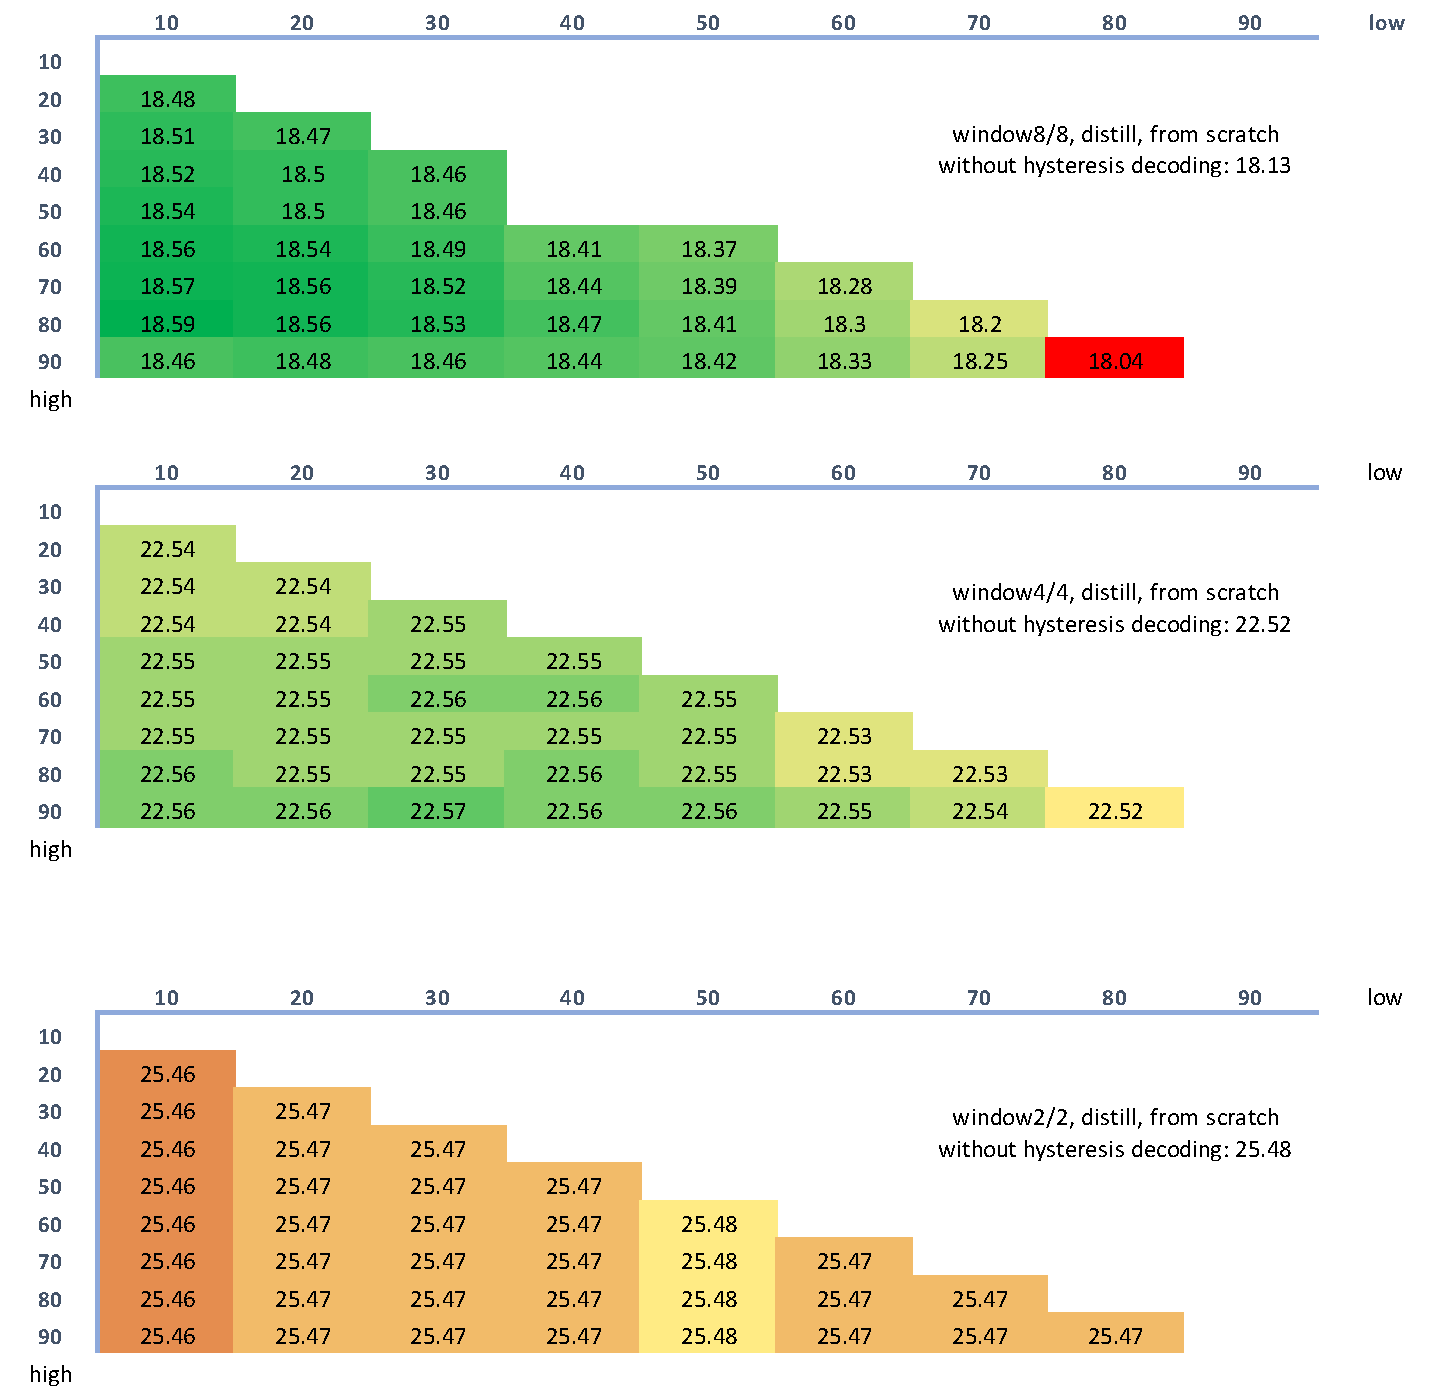
\includegraphics[width=\textwidth]{images/chap04_images/hysteresis_decoding_manual_2.pdf}
    \caption{Color coded lower triangular grid containing the BLEU4 score when decoding using a variety of low and high hysteresis thresholds for models trained from scratch. The darker the green/red, the better/worse the change in BLEU score. For example, for a window size of 8 each for past and future n-gram prediction window, trained on distilled data and from scratch, scored a BLEU4 score of 18.48 on a low threshold of 10 and a high threshold of 20 using hysteresis decoding. Without hysteresis decoding, the BLEU4 score is 18.13}
    \label{fig:hysteresis_decoding_manual_2}
\end{figure}
\begin{figure}[hpbt!]

    \centering
    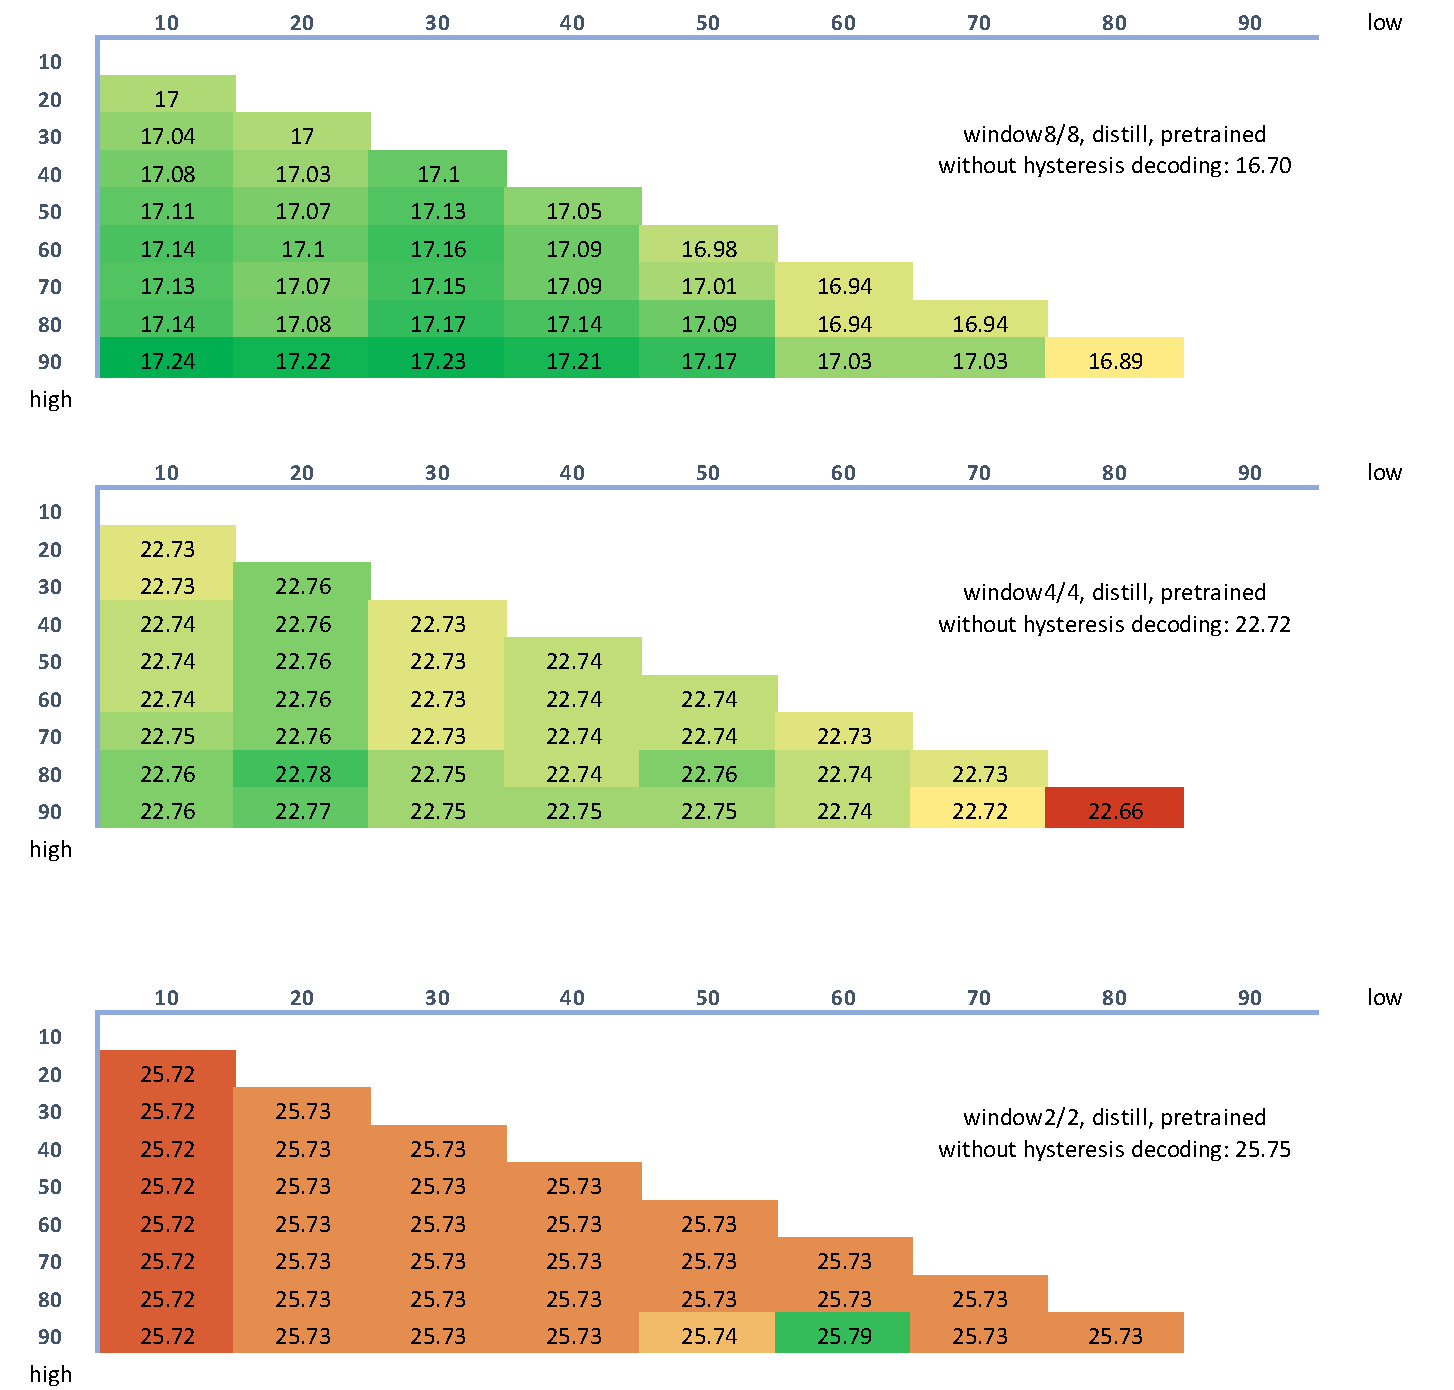
\includegraphics[width=\textwidth]{images/chap04_images/hysteresis_decoding_manual_1.pdf}
    \caption{Color coded lower triangular grid containing the BLEU4 score when decoding using a variety of low and high hysteresis thresholds for models trained from a pretrained model. The darker the green/red, the better/worse the change in BLEU score. For example, for a window size of 8 each for past and future n-gram prediction window, trained on distilled data and from scratch, scored a BLEU4 score of 17 on a low threshold of 10 and a high threshold of 20 using hysteresis decoding. Without hysteresis decoding, the BLEU4 score is 16.70}
    \label{fig:hysteresis_decoding_manual_1}
\end{figure}


We run a lower triangular grid search of low probabilities of 0.1 to 0.8, and high probabilities of 0.2 to 0.9, all in intervals of 0.1. Our results are shown and color coded in both Figure \ref{fig:hysteresis_decoding_manual_2} and Figure \ref{fig:hysteresis_decoding_manual_1}. Note that when using manual settings for hysteresis decoding, the probability of the candidate token is largely ignored, and the probability histories are used as basis for replacement.

Similar to the observations in Section \ref{subsubsec:range_hdec}, we deduce that the benefits of hysteresis decoding are more pronounced as the window sizes get larger, and its benefits are diminished for smaller window sizes. At window size of 8/8, there is a clear increase of the improvement in BLEU score compared to window 2/2, and 4/4. There is also a noticeable improvement in BLEU score as the difference between low and high threshold increases. This suggests the decoding process benefits from using surrounding tokens as a scaffolding to gauge the legitimacy of the generated token.

\subsection{Influence of freezing certain layers for transfer learning}
In order to understand the importance of the information in each layer to non-autoregressive sequence generation, we tried freezing different layers during transfer learning to determine the impact of training these layers. We conduct our experiments using a window size of 1/1 for the past-future ngram prediction task.

\subsubsection{Effect of freezing the encoder}

\begin{table}[]
\begin{tabular}{c|c|c|c|c|c|c|}
\cline{2-7}
                                     & \multicolumn{6}{c|}{Trainable Decoder Layer(s)}                          \\ \cline{2-7} 
                                     & 0, 1, 2, 3, 4, 5 & 1, 2, 3, 4, 5 & 2, 3, 4, 5 & 3, 4, 5 & 5, 4   & 5     \\ \hline
\multicolumn{1}{|c|}{frozen encoder} & 7.29             & 6.99          & 6.71       & 6.01    & 4.97   & 3.51  \\
\multicolumn{1}{|c|}{\% change}      & -73.43           & -74.52        & -75.54     & -78.09  & -81.88 & -87.2 \\ \hline
\end{tabular}
\caption{BLEU4 and percentage decrease in BLEU4 score when freezing the encoder and updating the decoder. These models use a window size of 1/1.}
\label{tab:freeze_encoder_results}
\end{table}

We freeze the encoder by not allowing any updates on the weights of the encoder during training. The decoder is still trained and updated as normal. 

Our results are shown at Table \ref{tab:freeze_encoder_results}. We find that freezing the encoder resulted in a catastrophic drop in performance. Therefore, we focus on freezing different layers in both the decoder and the encoder.


% \subsubsection{Effect of freezing the decoder}
% We train the encoder and freeze the decoder by not allowing the weights of the decoder to be updated during training. We find that freezing the 

\subsubsection{Importance of the position of trained layers for transfer learning}

\begin{table}[]
\centering
\begin{tabular}{c|c|c|c|}
\cline{2-4}
\multicolumn{1}{l|}{}            & \multicolumn{3}{c|}{Layers trained} \\ \cline{2-4} 
                                 & d05e05   & d0145e0145  & d5e012345  \\ \hline
\multicolumn{1}{|c|}{window 1/1} & 18.76    & 23.37       & 23.21      \\
\multicolumn{1}{|c|}{\% decline} & -31.63   & -14.83      & -15.42     \\ \hline
\multicolumn{1}{|c|}{window 2/2} & 14.79    & 19.66       & 19.9       \\
\multicolumn{1}{|c|}{\% decline} & -42.56   & -23.65      & -22.72     \\ \hline
\multicolumn{1}{|c|}{window 4/4} & 7.62     & 13.62       & 17.11      \\
\multicolumn{1}{|c|}{\% decline} & -66.46   & -40.05      & -24.69     \\ \hline
\end{tabular}
\caption{Decline in BLEU4 score when freezing certain layers. For example, d5e012345 means that the 5th layer of the decoder and the layers 0-5 of the encoder are trained, and the rest of the layers (layer 0-4 of the decoder) are frozen.}
\label{tab:freeze_layers_results}
\end{table}


For adapting autoregressive models to non-autoregressive models, we find that choosing the right layers to train is more important than the actual number of layers train. For instance, we find that the encoders' layers are the most important layers to be trained. we can freeze most of the decoder layers and minimize the impact on the BLEU4 score. We also find the layers closer to the input and output are the most important layers to be trained. Our results are shown in Table \ref{freeze_layers_results}

\textcite{ethayarajh-2019-contextual_ani} showed in their experiments that contextualized representations are anisotrophic in all inputs layers and higher layers. That means that the representations occupy a narrow cone in the vector space. We hypothesize that the anisotrophic property is not beneficial for non-autoregressive sequence generation. We leave the testing of this hypothesis up to future work.